% sets default font to Arial
\renewcommand{\rmdefault}{phv} % Arial
\renewcommand{\sfdefault}{phv} % Arial\\

%font size, document type and paper size
\documentclass[11pt,a4paper]{article}

\title{CMEE Miniproject}
\date{05 March 2019}
\author{Katherine Bickerton}

\usepackage[left=2cm,right=2cm,top=2cm,bottom=2cm]{geometry} % set page margins
\usepackage{lineno} % select specific line spacing
\linespread{1.5}\usepackage{pgfplotstable} % generate tables
\usepackage{graphicx} % inserting graphics
\usepackage{float} % positioning images
\usepackage[export]{adjustbox}
\usepackage{subcaption} % allow multiple figures
\usepackage{titlesec} % generate title page
\titleformat*{\section}{\large\bfseries}
\titleformat*{\subsection}{\normalsize\bfseries}
\usepackage{amsmath} % equation formatting
\usepackage{amssymb} % symbols for equations
\usepackage[round]{natbib} % generate biblography
\bibliographystyle{unsrtnat} % specific style of bibliography

\begin{document}
	
	\begin{titlepage}
		\centering
		\topskip2cm
		
\includegraphics[width = 7cm,left]{../Data/imperial_logo.png}
		{\Large
			\vskip2cm
			Using localised movements to examine the behaviour of two commercially important shark species in Western Australia.
		}    
		\vskip1cm	
		{\large Katherine Bickerton\\
		Submitted: August 2019}
		\vskip2cm	
		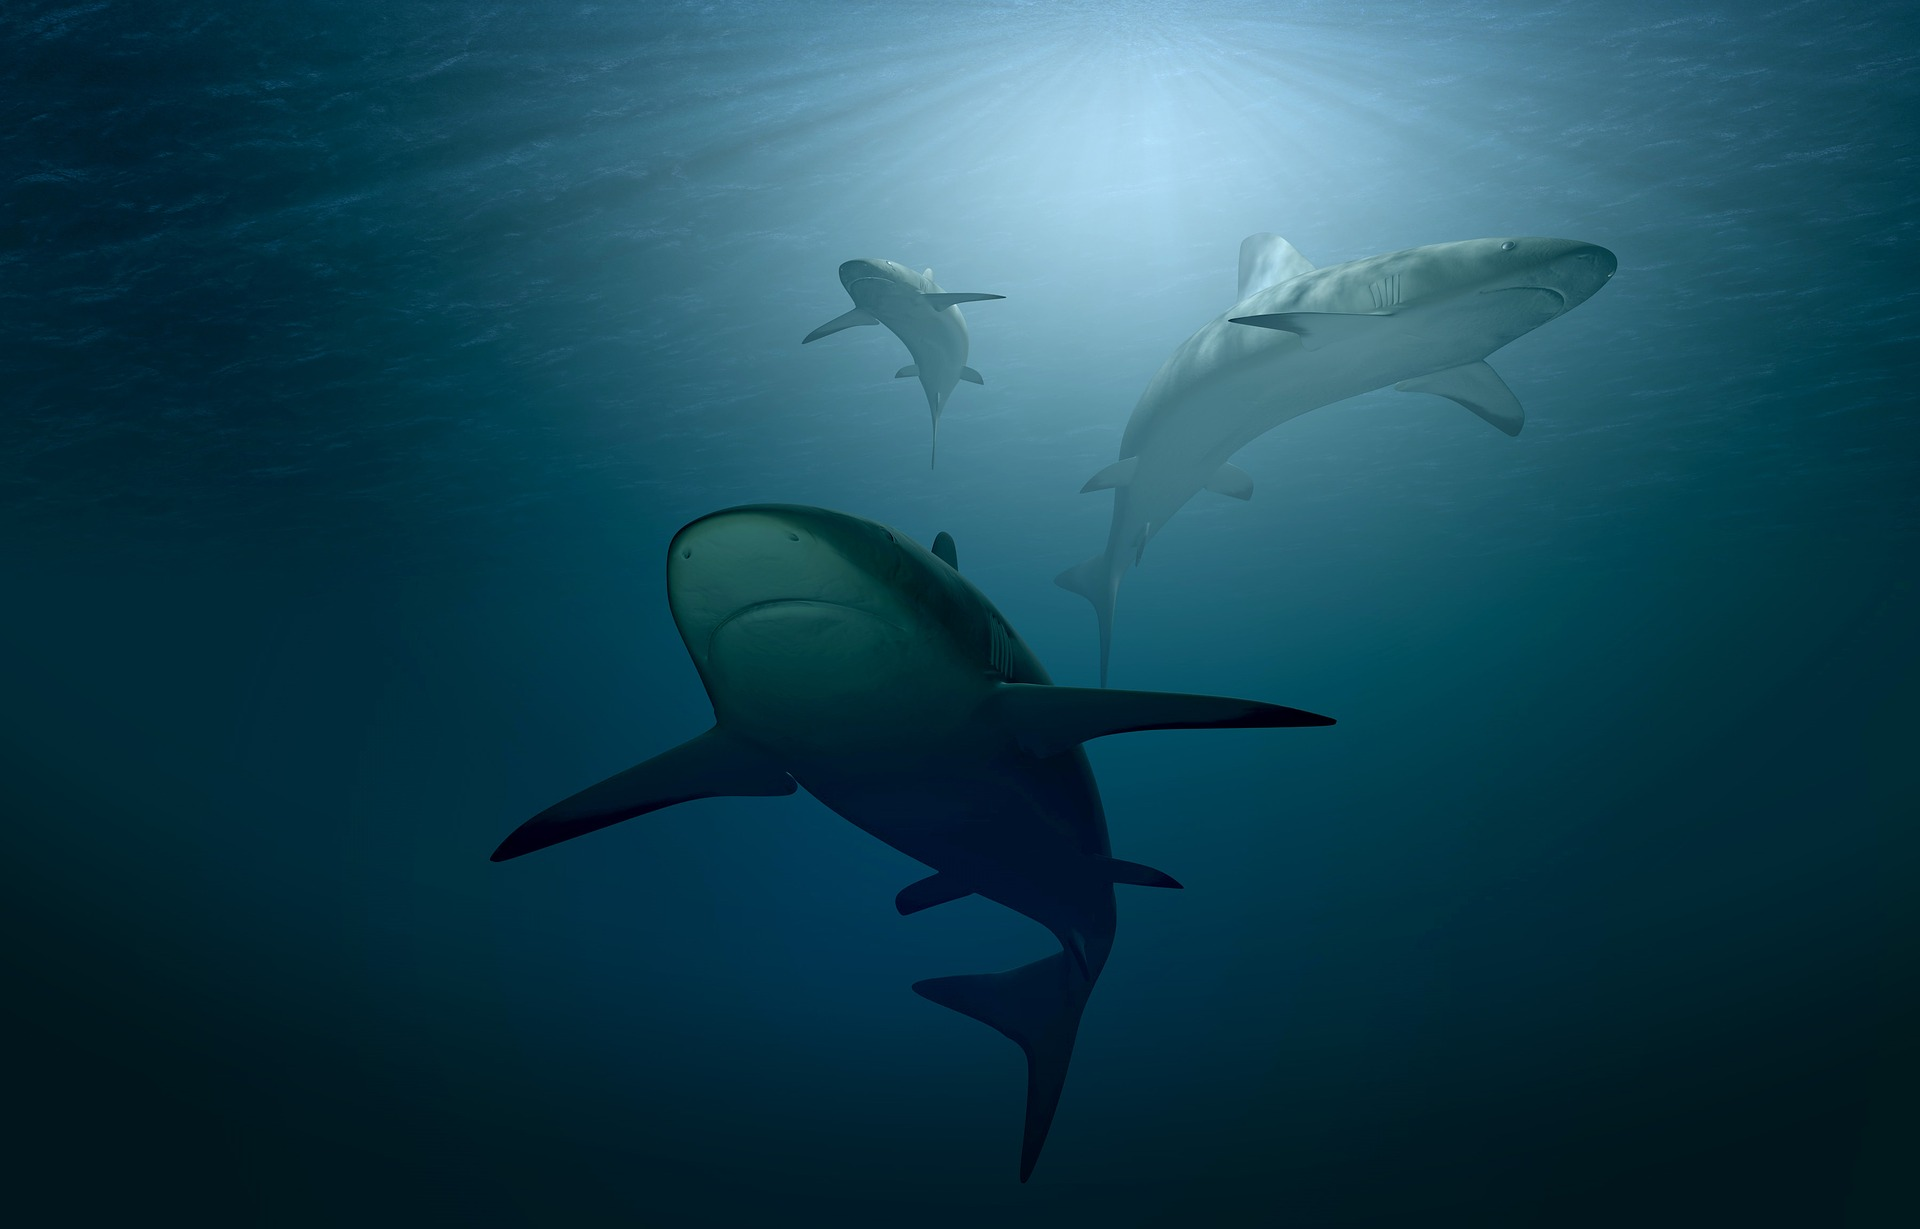
\includegraphics[width = 0.8\textwidth]{../Data/cover_image.jpg}
		\vskip4cm		
		\textbf{A thesis submitted in partial fulfilment of the requirements for the degree of Master of Research at Imperial College London\\
		Formatted in the journal style of the Marine Ecology Progress Series\\
		Submitted for the MRes in Computational Methods in Ecology and Evolution\\}
		\vspace*{\fill}
		\vspace*{\fill}
	\end{titlepage}
	
	
	\newpage
	
	\pagenumbering{gobble}
	\noindent{\large \textit{Declaration}}\\
	
	\noindent
	I declare that the data used in this project was collected and provided by my secondary supervisor Dr Matias Braccini, Western Australian Fisheries and Marine Laboratories, Government of Western Australia. I was provided with the raw dataset and carried out all processing, analysis and model development myself, with advice from Dr Matias Braccini and my primary supervisor, Dr David Jacoby, Institute of Zoology, Zoological Society of London. Dr Jacoby also provided training and R code for network analysis, which I adapted for the dataset used.
	
	
	
	
	\newpage
	\pagenumbering{arabic}
	
	\section{Abstract}
	
	
	\newpage
	
	\section{Introduction}
	
	\newpage
	
	\section{Methods \& Materials}
	
	\newpage
	
	\section{Results}
	
	\newpage
	
	\section{Discussion}
	
	\newpage
	
	\noindent{\large \textit{Acknowledgements}}
	
	\noindent{\large \textit{Data \& Code Availability}}
	
	\newpage
	
	\section{References}
	
	\newpage
	
	\section{Supplementary Information}
	
	
	
	
	
	
\end{document}